\documentclass{article}
\usepackage{graphicx} % Required for inserting images
\usepackage{kotex}
\usepackage{minted} % 소스 코드 하이라이팅
\usemintedstyle{friendly}

\title{프로그래밍언어론 hw5}
\author{C011013 권찬}
\date{2024.06.12}

\begin{document}

\maketitle

\section{Prolog}
\quad Prolog는 1973년 프랑스의 알랭 코메르가 개발한 논리형 언어입니다.\\
논리식을 사용하여 오브젝트와 오브젝트 사이의 관계에 대한 문제를 해결하기 위해 사용합니다.\\

\subsection{Prolog 특징}
1. Symbolic Programming\\
\quad Prolog는 수치연산보다 심볼 연산에 특화된 언어이므로, 수치 연산에 대한 언어적 지원이 약합니다. 대신 심볼 연산 구현은 다른 언어보다 깔끔하게 표현할 수 있습니다.\\\\
2. Declarative Programming\\
\quad Prolog는 선언적 패러다임으로 대부분의 절차적 언어와는 달리 같은 문제에 대해 다른 해결방법을 강제합니다.\\\\
3. Logic Programming\\
\quad 논리를 프로그래밍 언어로 표현합니다.

\subsection{Prolog 구성 요소}

1. 사실\\
\quad 객체가 갖고 있는 관계 하나를 true로 정의합니다.\\
관계와 객체의 이름은 소문자로 시작하며, 관계의 이름을 먼저 쓰고, 객체들은 괄호 안에 쉼표로 구분합니다.\\
모든 사실은 마침표(.)로 끝납니다.\\
\begin{minted}[frame=single, framesep=10pt, breaklines=true, fontsize=\small, linenos=true]{c}
fruit(apple).      // apple은 'fruit' 라는 특성을 갖는다.
likes(Jhon, Mary). // Jhon, Mary 는 '좋아한다' 라는 관계를 갖는다.
\end{minted}
2. 규칙\\
사실과 사실 사이에 관계를 정의하여, 주어진 사실들로 다른 사실을 추론할 수 있게 합니다.\\
Head :- Body 형식으로 작성하며, Head는 추론할 (확인할) 다른 사실을 가리키며, Body 에는 이를 추론하는데 사용할 다른 사실들이 들어갑니다.\\
\begin{minted}[frame=single, framesep=10pt, breaklines=true, fontsize=\small, linenos=true]{c}
sweet(Var) :- fruit(Var).      // Var이 과일이라면 (즉, fruit(Var) 이 true 라면) Var은 달다. (즉, sweet(Var)도 true 이다.)
\end{minted}
이때 새로운 사실을 추론할 기존 사실들은 여러 사실들이 들어갈 수 있습니다.\\
\begin{minted}[frame=single, framesep=10pt, breaklines=true, fontsize=\small, linenos=true]{c}
P :- Q, R.  // Q 와 R 이 모두 true 이면 P 도 true 이다.
P :- Q; R.  // Q 가 참이면 P도 true 이다. (R은 확인하지 않는다.) 만약 Q가 거짓이라면, R을 확인하고 R이 true이면 P도 true이다.
\end{minted}
Q가 참이면 R을 확인하지 않고, Q가 거짓일 때만 R을 확인한다는 점에서 일종의 if-else 문처럼 사용할 수 있습니다.\\\\
3. 질문\\
어떤 관계에 대한 사실을 질문합니다. 기존 사실들과 규칙으로부터 해당 관계에 대한 사실의 true, false 여부를 판단합니다.
\begin{minted}[frame=single, framesep=10pt, breaklines=true, fontsize=\small, linenos=true]{c}
? - sweet(apple).
true.
\end{minted}


\section{과제 코드 작동 방식}

\subsection{hw5a: Insertion Sort}

\subsubsection{알고리즘 및 구현}
\quad Insertion Sort 알고리즘은 0번째 인덱스부터 하나씩 증가하면서 key를 선정합니다.\\
현재 단계에서 키를 선정했다면, 해당 키 값보다 앞에 있는 리스트는 정렬이 되어있습니다.\\
따라서 해당 키를 자신 앞에 있는 정렬된 리스트 안에 정렬이 지켜지도록 적절한 위치에 끼워넣습니다.\\
이 과 정을 전체 key에 대해서 반복하면 전체 리스트를 정렬할 수 있습니다.\\
이때 선택한 key를 앞에 있는 리스트에 끼워 넣으면, 끼워넣은 위치 이후의 모든 원소가 뒤로 한 칸씩 밀려야 합니다.\\
이를 고려하여, 키를 끼워넣을 때는 자신 바로 직전에 있는 원소와 자신을 비교하여, 자신이 더 작으면 swap 하고, 그렇지 않으면 멈추는 과정을 수행합니다.\\\\
\textbf{1. sorting 함수}
\begin{minted}[frame=single, framesep=10pt, breaklines=true, fontsize=\small, linenos=true]{c}
sorting(Input, Result):-
  solve(Input, 0, Result), % 0은 시작할 초기 key index
  nl.
\end{minted}
Prolog의 모든 규칙은 일종의 함수로 생각할 수 있습니다. 과제 설명 보고서에는 함수로 표기하겠습니다.\\
과제 예시에서 나온대로, 문제를 해결할 sorting 함수를 작성하였습니다.\\
이 함수는 정렬할 배열을 첫번째 매개변수 Input 으로 받고, 그 결과를 받을 변수를 두번째 매개변수 Result로 받습니다.\\
내부적으로는 solve() 함수를 호출합니다. 이때 solve 함수는 Input, Result 외에도 정렬을 시작할 기준 key index를 0으로 초기화하여 호출합니다.\\\\
\textbf{2. solve 함수}
\begin{minted}[frame=single, framesep=10pt, breaklines=true, fontsize=\small, linenos=true]{c}
solve(Input, KeyIndex, Result):-
  length(Input, InputSize),   % Input 배열의 길이 계산, 이 길이까지만 key 인덱스를 증가시키기 위함.
  ( KeyIndex =:= InputSize -> (   % Input 배열의 길이와 key 인덱스가 같다면
      var(Result),                %   Result 변수가 할당되지 않았는지 체크하고
      Result = Input              %   할당되지 않았다면 Input 에는 정렬된 배열이 들어있으니 Result에 할당
    ) ; (                         % Input 배열의 길이 > key 라면
      InsertStartIndex is KeyIndex - 1, % key index 직전 인덱스부터, 그 값을 비교한다.
      insert(Input, InsertStartIndex, KeyIndex, SwapResult), % 현재 key값을 자신 앞에 있는 배열에 정렬되도록 끼워넣는다.

      write(KeyIndex),  % 현재 몇번째 키를 보고 있었는지 출력
      write(' '),
      writeln(SwapResult), % 현재 단계에서 정렬된 상태 출력

      NewKeyIndex is KeyIndex + 1, % 다음 키에 대해 반복하기 위해 key index 증가
      solve(SwapResult, NewKeyIndex, Result) % 다음 키에 대해서 sovle 반복 수행
    )
  ).
\end{minted}
solve 함수가 실행되면 제일 먼저 length 내장 함수를 이용하여 Input 으로 들어온 배열의 길이를 계산합니다. 이때 Input은 keyIndex 이전 인덱스까지는 정렬된 배열을 가리킵니다.\\
만약 Input 길이와 현재 keyIndex를 비교해서 그 값이 같다면 모든 key를 다 순회한 것이므로 반복(재귀)를 멈추고 Result 변수에 정렬된 결과 (Input) 을 저장합니다.\\
만약 KeyIndex < InputSize 이면 KeyIndex 직전 인덱스부터 0번 인덱스까지 반복하면서 Key값을 적절한 위치에 삽입합니다. 이 과정은 insert() 함수가 수행하도록 하였으며, 뒤에서 설명하겠습니다.\\
insert() 함수가 현재 키 값을 적절히 끼워넣어서 현재 단계의 정렬을 마쳤다면 현재 단계로서 KeyIndex를 출력하고, 정렬된 결과로 SwapResult를 출력합니다.\\
이제 다음 key에 대해 정렬을 수행하기 위해 KeyIndex를 1 증가시킨 NewKeyIndex와 중간 정렬된 배열 SwapResult를 solve 함수에 넘겨 재귀적으로 호출합니다.\\\\
\textbf{3. insert 함수}
\begin{minted}[frame=single, framesep=10pt, breaklines=true, fontsize=\small, linenos=true]{c}
insert(Input, NowIndex, KeyIndex, Result):- % Input 은 KeyIndex 이전까지는 정렬된 배열, NowIndex 위치에 KeyIndex를 삽입할 수 있는지 확인한다. 초기 호출 시 NowIndex 값은 KeyIndex - 1 이다.
  (NowIndex < 0 -> ( % NowIndex 가 0보다 작다면 key index 이전의 모든 배열을 순회한 것이므로 반복(재귀)를 종료한다.
      Result = Input % 그리고 삽입한 최종 결과 배열을 Result에 저장한다.
    ) ; (  % NowIndex가 0보다 크다면
      nth0(KeyIndex, Input, KeyValue), % KeyValue = Input[KeyIndex]
      nth0(NowIndex, Input, NowValue), % NowValue = Input[NowIndex]
      (KeyValue < NowValue -> (
          swap(Input, NowIndex, KeyIndex, SwapResult), % KeyValue < NowValue 이면 두 값을 스왑하고
          NextKeyIndex is KeyIndex - 1                 % KeyValue가 앞으로 갔으니 NextKeyIndex에 KeyIndex - 1 대입
        ) ; (
          SwapResult = Input,       % 만약 스왑을 하지 않았더라도, SwapResult 변수에 Input을 그대로 넣기
          NextKeyIndex is KeyIndex  % NextKeyIndex 에는 KeyIndex 그대로 유지
        )
      ),
      NextIndex is NowIndex - 1, % 다음 반복에서 Key와 비교할 Index 값.
      insert(SwapResult, NextIndex, NextKeyIndex, Result) % 다음 반복 진행
    )
  ).
\end{minted}
insert함수는 현재까지 정렬된 배열을 Input으로, 현재 반복(재귀단계)에서 삽입할지 여부를 체크할 위치를 NowIndex로, 현재 key 의 위치를 KeyIndex로, 삽입된 최종 결과를 저장할 Result 변수를 매개변수로 갖습니다.\\
만약 NowIndex < 0 이면 모든 인덱스에 대해 삽입여부를 체크한 것이므로 Result에 그때까지 삽입이 완료된 Input을 대입하고 종료합니다.\\
만약 NowIndex > 0 이면 KeyValue, NowValue 변수에 KeyIndex, NowIndex 위치에 있는 값을 nth0 내장함수를 이용해 Input에서 읽어와 대입합니다.\\
대입된 값을 비교해서 KeyValue < NowValue 이면 swap을 진행합니다. swap 역시 별도 함수로 구현하였으며, 뒤에 후술하겠습니다.\\
만약 KeyValue >= NowValue 이면 swap하지 않고 다음 단계로 넘어갑니다.\\
이 과정을 거치면 현재 key 인덱스를 자신 앞쪽에 적절히 삽입한, 현재 단계에서 key index까지 정렬된 결과를 얻을 수 있습니다.\\\\
\textbf{4. swap 함수}
\begin{minted}[frame=single, framesep=10pt, breaklines=true, fontsize=\small, linenos=true]{c}
swap(Input, CheckIndex, KeyIndex, Result):-
  % CheckIndex < KeyIndex 가 전제 되어야 nth0/4 로 삽입, 추출이 꼬이지 않음.
  nth0(KeyIndex, Input, KeyValue, RestInput),           % KeyIndex 위치에 있는 값을 KeyValue에 저장하고, Input에서 그 값을 뽑아낸 나머지 배열을 RestInput에 저장
  nth0(CheckIndex, RestInput, CheckValue, RestInput2),  % RestInput에서 CheckIndex 위치에 있는 값을 CheckValue에 저장하고, 그 값을 뽑아낸 나머지 배열을 RestInput2에 저장
  nth0(CheckIndex, SwapResult1, KeyValue, RestInput2),  % RestInput2에 KeyValue를 CheckIndex 위치에 삽입하고, 그 결과를 SwapResult1 에 저장
  nth0(KeyIndex, Result, CheckValue, SwapResult1).      % SwapResult1에 CheckValue를 KeyIndex 위치에 삽입하고, 그 결과를 Result 에 저장
\end{minted}
swap은 nth0 내장 함수를 이용하여 진행하였습니다.\\
nth0 내장함수는 0-index 기준으로 다음과 같이 동작합니다.\\\\
- nth0(Index, List, Value, SubList) : List에서 Index위치에 있는 값을 빼고 Value 에 저장합니다. Value가 빠지고 남은 리스트를 SubList에 저장합니다. 이 경우엔 Value, SubList에 결과물이 저장됩니다.\\
만약 List에 변수를 두고, Index, Value, SubList에 값을 넘기면, SubList에서 Index위치에 Value를 삽입한 결과를 List로 돌려줍니다.\\\\
이를 이용하면 다음 과정으로 swap을 구현할 수 있습니다. \\
1. Input 에서 KeyValue를 뺍니다. KeyValue가 CheckValue보다 뒤에 있기 때문에 Key를 먼저 빼야 나중에 인덱스가 꼬이지 않습니다.\\
Input에서 KeyValue를 빼고 남은 리스트는 RestList에 저장됩니다.\\
2. 남은 RestList에 대해서 CheckIndex 위치에 있는 CheckValue를 빼고, 그 결과를 RestList2에 저장합니다.\\
RestList2에는 CheckValue, KeyValue 2개가 모두 빠져있습니다.\\
3. RestList2에 KeyValue를 CheckIndex 위치에 삽입합니다. 그 결과를 SwapResult1에 저장합니다.\\
4. SwapResult1에 CheckValue를 KeyIndex 위치에 삽입합니다. 그 결과를 Result에 저장합니다.\\\\
\subsubsection{실행 결과}
\begin{figure}[!htb]
    \centering
    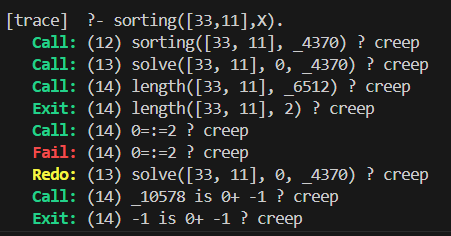
\includegraphics[width=0.8\linewidth]{hw5a_1.png}
\end{figure}
[33, 11] 을 정렬하는 과정을 trace로 따라가보겠습니다.\\
먼저 sorting 함수를 실행하면, 다음으로 solve 함수가 실행됩니다.
배열의 길이를 구하려고 length 함수를 실행하여 길이를 구하면 2가 나오고, 이 값은 현재 체크하는 키 값인 0보다 크므로, insert 하는 코드가 실행됩니다.\\
\begin{figure}[!htb]
    \centering
    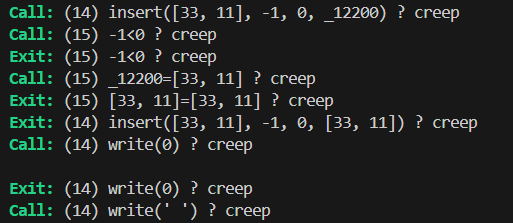
\includegraphics[width=0.8\linewidth]{hw5a_2.png}
\end{figure}\\
insert 함수가 실행되면 현재 key index가 0이므로, InsertStartIndex에는 -1이 들어갑니다.\\
insert 함수에서는 NowIndex 가 -1 < 0 이므로 함수의 실행을 종료하고, insert 결과로 Input을 그대로 돌려줍니다.\\
\newpage
\begin{figure}[!htb]
    \centering
    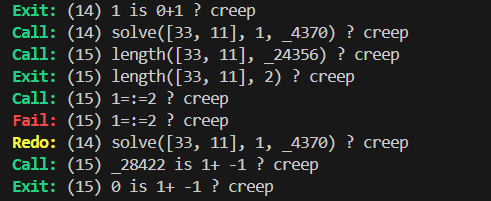
\includegraphics[width=0.8\linewidth]{hw5a_3.png}
\end{figure}
현재 단계의 solve가 종료되고, key index를 1 증가해서 solve 함수를 호출합니다.\\
solve함수가 실행되면 똑같이 length를 구한 뒤 비교하고, insert 함수가 실행됩니다.\\
\begin{figure}[!htb]
    \centering
    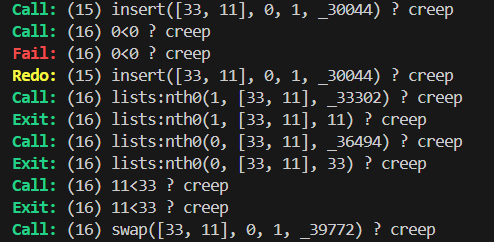
\includegraphics[width=0.8\linewidth]{hw5a_4.png}
\end{figure}\\
이번에는 두 인덱스로부터 값을 읽은 뒤 비교합니다. key 값이 이전 인덱스의 값보다 작으므로 swap 함수가 호출됩니다.\\
\begin{figure}[!htb]
    \centering
    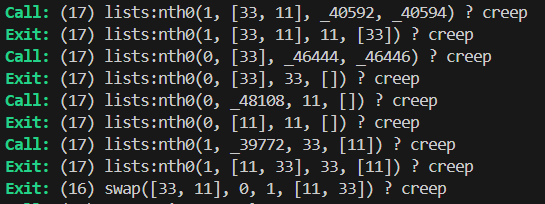
\includegraphics[width=0.8\linewidth]{hw5a_5.png}
\end{figure}\\
그러면 위에서 설명한 과정으로 swap이 진행됩니다. swap() 함수가 종료될 때, Result 변수에 담기는 값을 보면 swap이 되어있음을 알 수 있습니다.\\
\begin{figure}[!h]
    \centering
    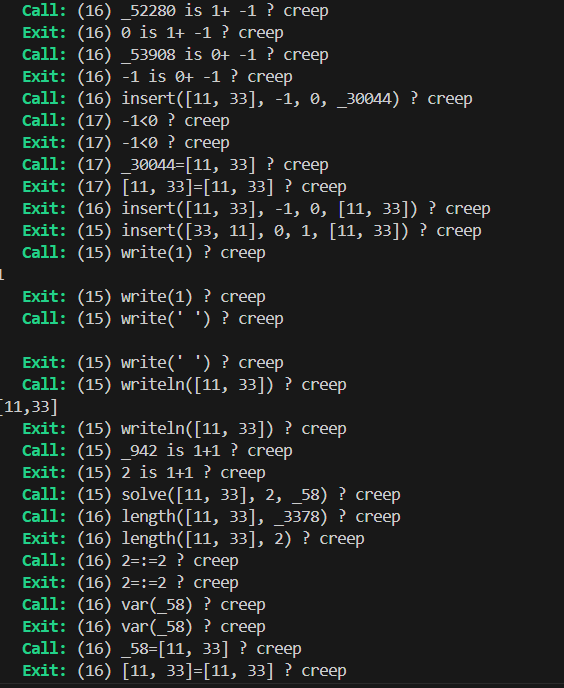
\includegraphics[width=0.8\linewidth]{hw5a_6.png}
\end{figure}\\
이후에는 insert가 -1 인덱스에 진행되어 반복이 종료되고, solve 함수도 key index == length 가 되어 Result변수에 최종 정렬된 배열을 담으면서 종료합니다.
\newpage
\begin{figure}
    \centering
    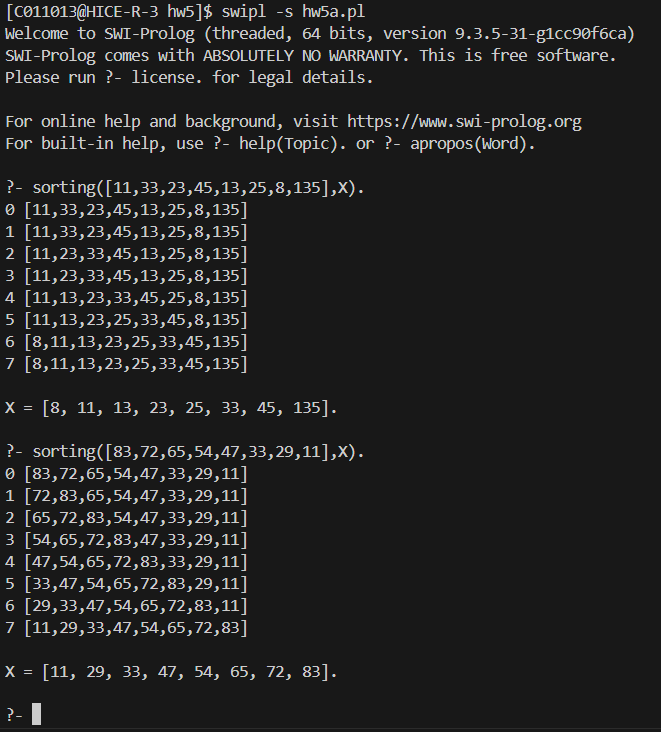
\includegraphics[width=0.8\linewidth]{hw5a_7.png}
\end{figure}
실행 결과는 위와 같습니다.
\subsection{hw5b: N-Queen}
\subsubsection{알고리즘}

\quad N-Queen 문제를 풀기 위해, 먼저 생각할 수 있는 것은, 퀸은 하나의 가로줄에 하나만 존재해야 한다는 것을 쉽게 떠올릴 수 있습니다.\\
하나의 가로줄에 여러 퀸이 있으면 서로가 서소를 가로 방향으로 공격할 수 있기 때문입니다.\\
따라서 각각의 가로줄마다 퀸을 임의 세로줄에 하나씩 배치해보면서 지금 가로줄에서 이 세로줄 위치에 퀸을 배치했을 때 서로 공격할 수 있는지 체크하고, 만약 공격할 수 있다면 그 세로줄에는 배치할 수 없으므로 그 케이스는 건너 뛰고, 배치할 수 있다면 그 위치에 일단 배치한 후, 다음 가로줄로 넘어가 이어서 퀸을 배치해봅니다.\\
위와 같이 일단 모든 경우의 수를 시도해보다가 중간에 안되는 경우를 만났을 때 뒤로 돌아가는 알고리즘을 백트래킹이라고 하며, 재귀를 이용해 구현할 수 있습니다.\\\\
\textbf{1. n\_queen 함수}
\begin{minted}[frame=single, framesep=10pt, breaklines=true, fontsize=\small, linenos=true]{c}
% N-Queen
n_queen(N, Result):- % Result에는 실행 결과로 퀸을 배치하는 방법 리스트가 출력
  solve(N, 1, 1, [], Result),
  nl.
\end{minted}
과제 예시에 맞추어 n\_queen 함수를 작성합니다. 보드의 크기 N과, 퀸을 배치한 결과를 받을 Result 변수를 매개변수로 갖습니다.\\
내부에서는 solve() 함수를 호출합니다.\\\\
\textbf{2. solve 함수}
\begin{minted}[frame=single, framesep=10pt, breaklines=true, fontsize=\small, linenos=true]{c}
solve(N, Line, Pos, Result, FinalResult):-
  ( N < Line -> (                                         % N < Line 이면, 모든 행에 퀸을 다 배치한 것이므로,
      var(FinalResult) ->                                 % FinalResult에 결과가 저장되어 있지 않다면 
        FinalResult = Result                              % FinalResult에 결과를 저장한다. (따라서 여러 경우의 수가 존재해도 1가지만 저장한다.)
      ;
        !                                                 % FinalResult에 이미 저장되어 있으면 무시한다.
    ) ; (
      Pos =< N -> (                                       % 만약 현재 배치하려고 하는 열이 N 이하라면 배치할 수 있으니
        check_line(Line, Pos, Result) ->                  % 이 행,열에 퀸을 새로 배치할 수 있는지 체크한다.
          NextLine is Line + 1,                           % 
          append(Result, [Pos], NewResult),               % 배치할 수 있으면, 배치 결과 리스트에 현재 행,열을 추가      
          solve(N, NextLine, 1, NewResult, FinalResult)   % 다음 행에 대해서 solve 진행
        ;
          true                                            % 이 위치에 배치할 수 없으면 무시. (재귀 종료)
        ),
        NextPos is Pos + 1,
        solve(N, Line, NextPos, Result, FinalResult)      % 현재 Pos에 대해 체크했으니 다음 Pos에 대해 체크하기
      ;                                                   % Pos > N 이면 범위를 벗어났으므로
        !                                                 % 재귀 종료
    )
  ).
\end{minted}
\quad solve함수는 N, Line, Pos, Result, FinalResult 를 매개변수로 갖습니다.\\
N은 보드판의 크기로서, Line, Pos의 반복범위를 체크하는 용도로 사용됩니다.\\
Line, Pos 는 퀸을 배치할 수 있는지 체크할 가로, 세로 위치입니다.\\
Result는 지금 solve를 호출하는 시점까지 배치한 퀸의 위치 리스트입니다.\\
FinalResult는 N개의 퀸을 모두 배치하면 최종적으로 반환할 결과 위치 리스트입니다.\\\\
현재 Line이 N보다 크면, 범위를 벗어난 상황인데, Line이 증가하는 조건은 해당 라인에 배치할 수 있는 위치가 있어서 퀸을 배치했을 때만 증가하므로 Line > N 이면 모든 퀸을 배치했다는 의미이므로 그 결과를 FinalResult에 저장합니다. 이때 결과가 여러개 나오더라도 하나만 저장하도록 FinalResult에 값이 할당되었는지 체크하고 할당하였습니다.\\\\
만약 Line <= N 일 때, Line은 범위에 존재하니, Pos를 체크합니다.\\
Pos역시 N범위 안에 있다면 해당 Line, Pos 위치에 퀸을 배치할 수 있는지 check\_line 함수로 체크합니다. 이 함수는 뒤에 설명합니다.\\
그 결과로 퀸을 배치할 수 있다는 것이 확인되면, 퀸을 배치하고 해당 위치 정보를 Result에 추가하여 NewResult를 얻습니다. 그리고 현재 다음 Line에 퀸을 배치하기 위해 Line을 증가시키고 Pos는 0부터 확인하도록 해서 solve 함수를 재귀적으로 호출합니다.\\\\
만약 현재 Line, Pos 에 배치할 수 없다면, 그 다음 Pos를 체크하기 위해 Pos를 1 증가시키고 solve 함수를 호출합니다.\\\\
\textbf{3. check\_line, check\_diagonals 함수}
\begin{minted}[frame=single, framesep=10pt, breaklines=true, fontsize=\small, linenos=true]{c}
% X 조합으로 퀸을 배치했을 때, Line에서 Pos가 0부터 Line까지에 대해 퀸을 배치할 수 있는지 확인
check_line(Line, Pos, []):- true.
check_line(Line, Pos, NowResult):-
  % 한 행에는 하나의 퀸만 배치하므로, 행은 체크할 필요가 없다.
  % 열이 겹치는지 체크할 때는 Pos가 NowResult에 들어있는지 확인한다.
  \+ member(Pos, NowResult),
  % 대각선에 다른 퀸이 있는지 체크한다.
  check_diagonals(Line, Pos, 1, NowResult).

check_diagonals(_, _, _, []).  % 빈 리스트이면 대각선에 다른 퀸이 없음
check_diagonals(Line, Pos, CheckLine, [R | Rs]) :-
    DiagonalOffset is abs(Line - CheckLine),        % 현재 배치한 퀸과, 현재 배치하려고 하는 위치의 대각선의 차이 계산
    DiagonalOffset =\= abs(Pos - R),                % 가로줄 간격의 절댓값과, 세로줄 간격의 절댓값이 달라야 배치할 수 있다.
    NextCheckLine is CheckLine + 1,
    check_diagonals(Line, Pos, NextCheckLine, Rs).  % 나머지 퀸들에 대해 재귀적으로 확인
\end{minted}
check\_line 함수는 현재 line, pos 에 퀸을 배치할 수 있는지 체크합니다.\\
우선 행의 경우, 각 행마다 퀸을 하나씩 배치해보고 있으므로 체크할 필요가 없습니다.\\
열의 경우, 결과 리스트에 배치한 퀸의 열 정보를 저장하므로, 현재 Pos가 결과 리스트에 존재하는지 확인하면 됩니다. 이때 member 내장 함수를 활용합니다.\\
마지막으로 대각선에 퀸이 존재하는지 확인합니다. 이는 check\_diagonals 함수를 사용합니다.\\\\
check\_diagonals 함수는 중간에 퀸을 배치한 결과 리스트를 돌면서 해당 위치와 현재 배치하려고 하는 위치의 가로간격과 세로간격을 계산합니다. 그 두 간격의 절댓값이 동일하다면 대각선상 퀸이 존재하는 것이므로 배치할 수 없습니다.
\subsubsection{실행과정}
\begin{figure}[!htb]
    \centering
    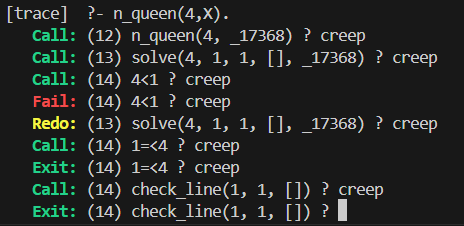
\includegraphics[width=0.8\linewidth]{hw5b_2.png}
\end{figure}
n\_queen 함수가 호출되면 내부에서는 solve함수가 호출됩니다.\\
현재 Line이 N 보다 작고, Pos도 N보다 작다는 것을 확인하면 현재 Line, Pos에 퀸을 배치할 수 있는지 check\_line 함수로 확인하기 위해 호출합니다.\\
\begin{figure}[!htb]
    \centering
    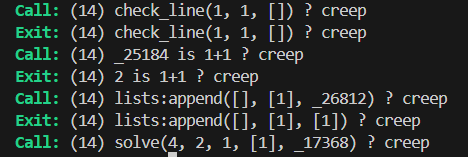
\includegraphics[width=0.8\linewidth]{hw5b_3.png}
\end{figure}\\
처음에는 리스트가 비어있으므로 바로 함수가 종료되고, 다음 Line에 대해 배치하기 위해 함수를 solve 함수를 재귀적으로 호출합니다.\\
\newpage
\begin{figure}[!htb]
    \centering
    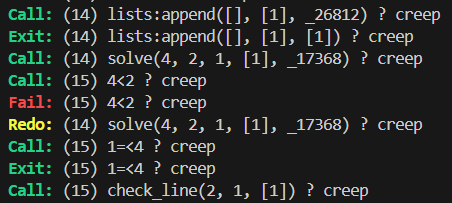
\includegraphics[width=0.8\linewidth]{hw5b_4.png}
\end{figure}
다음 함수를 재귀적으로 호출하기 전에 기존 [1,1]위치에 퀸을 배치했다는 정보를 리스트에 담고 호출합니다.\\
이제 다음 재귀에서는 [2,1] 위치를 체크합니다.
\begin{figure}[!htb]
    \centering
    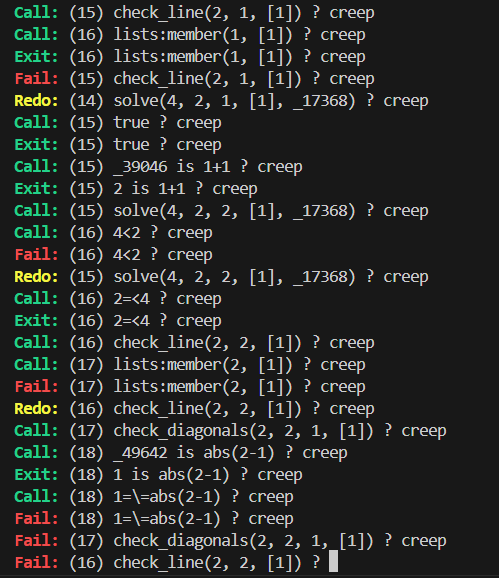
\includegraphics[width=0.8\linewidth]{hw5b_5.png}
\end{figure}\\
\quad [2,1], [2,2] 위치는 각각 행이 겹치고, 대각선이 겹치므로 배치할 수 없습니다.\\
따라서 check\_line 함수가 모두 실패합니다.\\
\newpage
\begin{figure}[!htb]
    \centering
    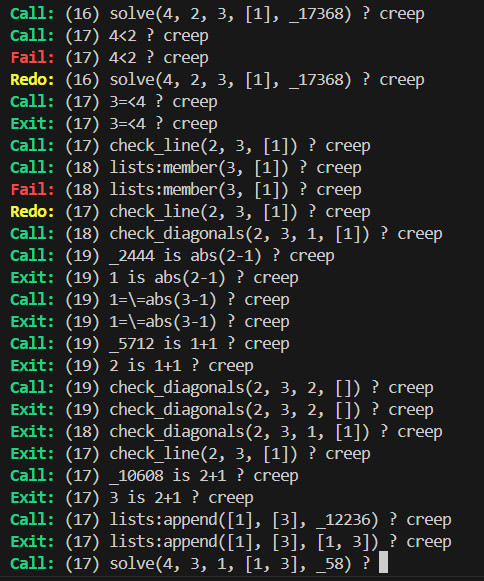
\includegraphics[width=0.8\linewidth]{hw5b_6.png}
\end{figure}
[2,3]은 이 과정을 모두 거쳤을 때 문제가 없는 위치이므로 결과 배열에 담고 다음 라인의 1번째 위치부터 solve 과정을 반복합니다.\\
이 과정을 반복하여 n\_queen 문제를 풀 수 있습니다.

\newpage

\subsubsection{실행결과}
\begin{figure}[!htb]
    \centering
    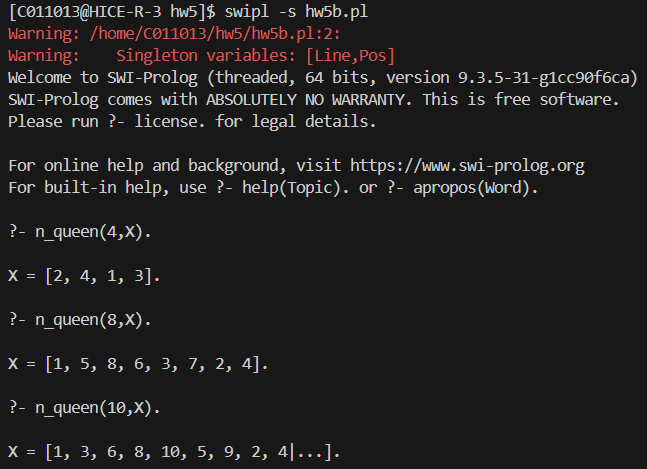
\includegraphics[width=0.8\linewidth]{hw5b_1.png}
\end{figure}

\section{어려웠던 점}
\quad 프롤로그 과제를 하면서 오히려 LISP 때보다 정말 함수형 언어를 사용하는 느낌이 들었습니다. 언어에 반복문이 존재하지 않아서 반복문을 재귀로 돌아야 하는 것이 매우 어색했습니다. 그리고 한변 변수에 값을 저장하면 그 값을 다시 덮어쓸 수 없는 점도 어려운 점 중 하나였습니다. 마지막으로 함수를 호출할 때 넘기는 매개변수가 함수를 호출할 때 인자를 넘기는 통로가 되기도 하고, 어떨때는 함수에서 생성한 결과값을 return 하는 통로로도 사용되는 점이 매우 어색해서 적응하기가 어려웠습니다.

\end{document}